\documentclass[14pt]{extbook}
\usepackage{multicol, enumerate, enumitem, hyperref, color, soul, setspace, parskip, fancyhdr} %General Packages
\usepackage{amssymb, amsthm, amsmath, bbm, latexsym, units, mathtools} %Math Packages
\everymath{\displaystyle} %All math in Display Style
% Packages with additional options
\usepackage[headsep=0.5cm,headheight=12pt, left=1 in,right= 1 in,top= 1 in,bottom= 1 in]{geometry}
\usepackage[usenames,dvipsnames]{xcolor}
\usepackage{dashrule}  % Package to use the command below to create lines between items
\newcommand{\litem}[1]{\item#1\hspace*{-1cm}\rule{\textwidth}{0.4pt}}
\pagestyle{fancy}
\lhead{Progress Quiz 9}
\chead{}
\rhead{Version A}
\lfoot{8590-6105}
\cfoot{}
\rfoot{Fall 2020}
\begin{document}

\begin{enumerate}
\litem{
Solve the rational equation below. Then, choose the interval(s) that the solution(s) belongs to.\[ \frac{5x}{7x + 5} + \frac{-4x^{2}}{-14x^{2} -59 x -35} = \frac{5}{-2x -7} \]\begin{enumerate}[label=\Alph*.]
\item \( \text{All solutions lead to invalid or complex values in the equation.} \)
\item \( x_1 \in [-6.71, -4.31] \text{ and } x_2 \in [-0.57,-0.28] \)
\item \( x \in [-3.61,-3.27] \)
\item \( x_1 \in [-6.71, -4.31] \text{ and } x_2 \in [-1,-0.57] \)
\item \( x \in [-1.16,0.71] \)

\end{enumerate} }
\litem{
Determine the domain of the function below.\[ f(x) = \frac{3}{24x^{2} -56 x + 30} \]\begin{enumerate}[label=\Alph*.]
\item \( \text{All Real numbers except } x = a, \text{ where } a \in [23.7, 25.5] \)
\item \( \text{All Real numbers except } x = a \text{ and } x = b, \text{ where } a \in [-0.8, 0.9] \text{ and } b \in [0.9, 3] \)
\item \( \text{All Real numbers except } x = a \text{ and } x = b, \text{ where } a \in [23.7, 25.5] \text{ and } b \in [29, 31.9] \)
\item \( \text{All Real numbers except } x = a, \text{ where } a \in [-0.8, 0.9] \)
\item \( \text{All Real numbers.} \)

\end{enumerate} }
\litem{
Solve the rational equation below. Then, choose the interval(s) that the solution(s) belongs to.\[ \frac{-36}{60x + 84} + 1 = \frac{-36}{60x + 84} \]\begin{enumerate}[label=\Alph*.]
\item \( \text{All solutions lead to invalid or complex values in the equation.} \)
\item \( x_1 \in [-3.4, -0.4] \text{ and } x_2 \in [0.4,2.4] \)
\item \( x \in [-2.4,-0.4] \)
\item \( x \in [0.4,2.4] \)
\item \( x_1 \in [-3.4, -0.4] \text{ and } x_2 \in [-3.4,0.6] \)

\end{enumerate} }
\litem{
Solve the rational equation below. Then, choose the interval(s) that the solution(s) belongs to.\[ \frac{42}{-30x + 24} + 1 = \frac{42}{-30x + 24} \]\begin{enumerate}[label=\Alph*.]
\item \( x \in [-0.2,1.8] \)
\item \( x \in [-1.5,-0.5] \)
\item \( \text{All solutions lead to invalid or complex values in the equation.} \)
\item \( x_1 \in [0.5, 1.3] \text{ and } x_2 \in [-1.2,2.8] \)
\item \( x_1 \in [-1.5, -0.5] \text{ and } x_2 \in [-1.2,2.8] \)

\end{enumerate} }
\litem{
Choose the graph of the equation below.\[ f(x) = \frac{-1}{x - 3} - 1 \]\begin{enumerate}[label=\Alph*.]
\begin{multicols}{2}\item 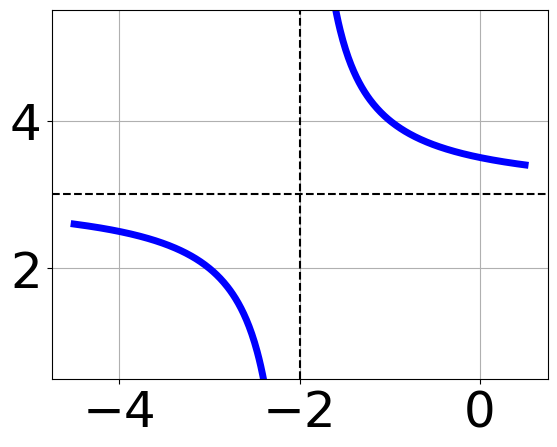
\includegraphics[width = 0.3\textwidth]{../Figures/rationalEquationToGraphCopyAA.png}\item 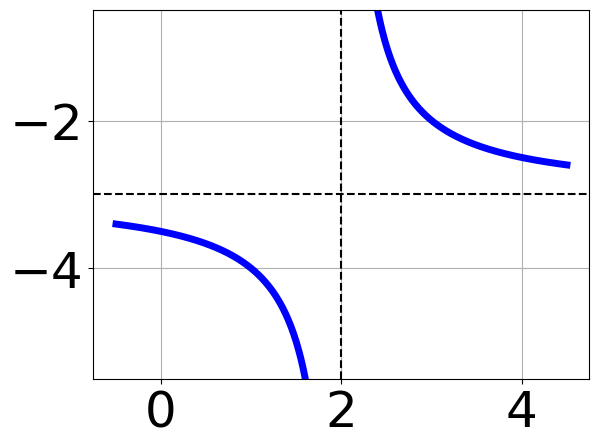
\includegraphics[width = 0.3\textwidth]{../Figures/rationalEquationToGraphCopyBA.png}\item 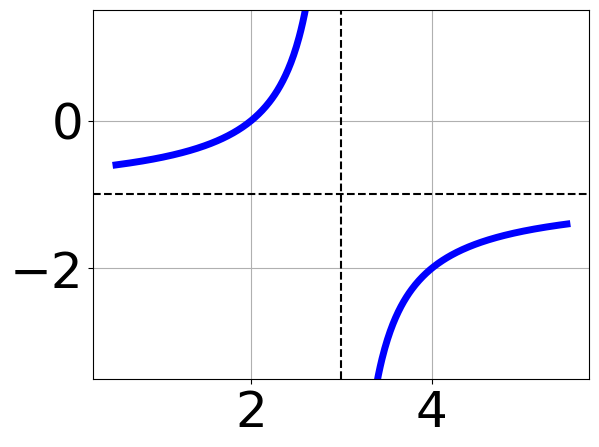
\includegraphics[width = 0.3\textwidth]{../Figures/rationalEquationToGraphCopyCA.png}\item 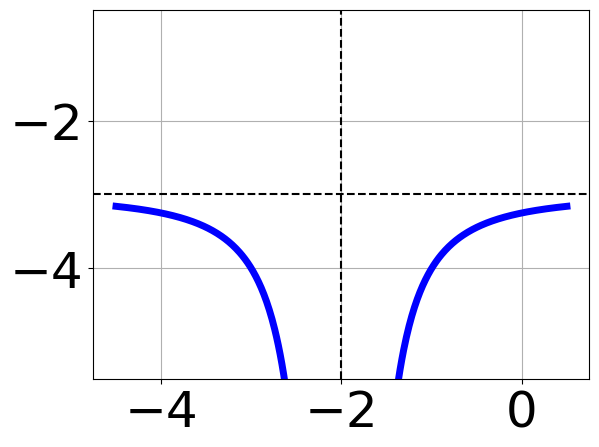
\includegraphics[width = 0.3\textwidth]{../Figures/rationalEquationToGraphCopyDA.png}\end{multicols}\item None of the above.
\end{enumerate} }
\litem{
Determine the domain of the function below.\[ f(x) = \frac{6}{12x^{2} +29 x + 15} \]\begin{enumerate}[label=\Alph*.]
\item \( \text{All Real numbers except } x = a, \text{ where } a \in [-16.7, -14.9] \)
\item \( \text{All Real numbers except } x = a \text{ and } x = b, \text{ where } a \in [-16.7, -14.9] \text{ and } b \in [-12.3, -11.6] \)
\item \( \text{All Real numbers.} \)
\item \( \text{All Real numbers except } x = a, \text{ where } a \in [-4, -1.5] \)
\item \( \text{All Real numbers except } x = a \text{ and } x = b, \text{ where } a \in [-4, -1.5] \text{ and } b \in [-1.6, 0.1] \)

\end{enumerate} }
\litem{
Choose the equation of the function graphed below.
\begin{center}
    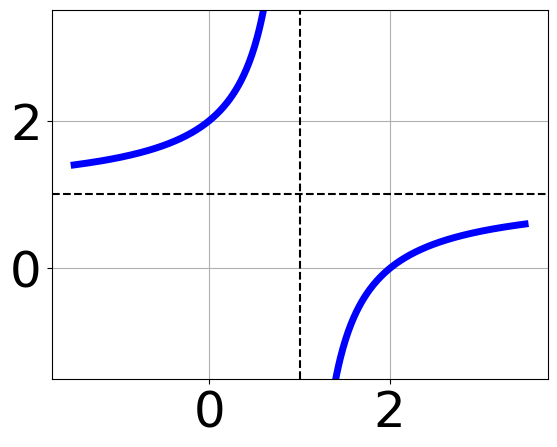
\includegraphics[width=0.5\textwidth]{../Figures/rationalGraphToEquationCopyA.png}
\end{center}
\begin{enumerate}[label=\Alph*.]
\item \( f(x) = \frac{-1}{(x - 2)^2} - 7 \)
\item \( f(x) = \frac{1}{(x + 2)^2} - 7 \)
\item \( f(x) = \frac{1}{x + 2} - 7 \)
\item \( f(x) = \frac{-1}{x - 2} - 7 \)
\item \( \text{None of the above} \)

\end{enumerate} }
\litem{
Choose the equation of the function graphed below.
\begin{center}
    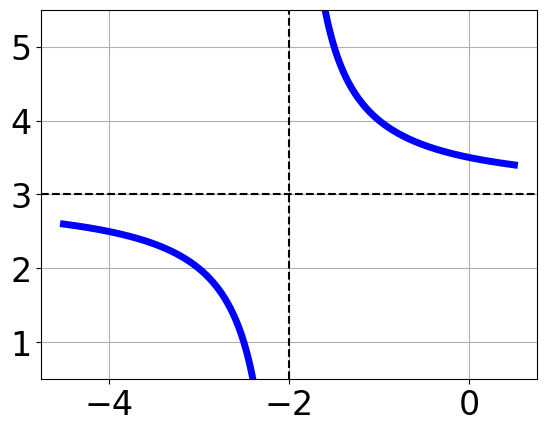
\includegraphics[width=0.5\textwidth]{../Figures/rationalGraphToEquationA.png}
\end{center}
\begin{enumerate}[label=\Alph*.]
\item \( f(x) = \frac{1}{(x + 3)^2} - 1 \)
\item \( f(x) = \frac{-1}{(x - 3)^2} - 1 \)
\item \( f(x) = \frac{1}{x + 3} - 1 \)
\item \( f(x) = \frac{-1}{x - 3} - 1 \)
\item \( \text{None of the above} \)

\end{enumerate} }
\litem{
Choose the graph of the equation below.\[ f(x) = \frac{-1}{x + 3} - 1 \]\begin{enumerate}[label=\Alph*.]
\begin{multicols}{2}\item 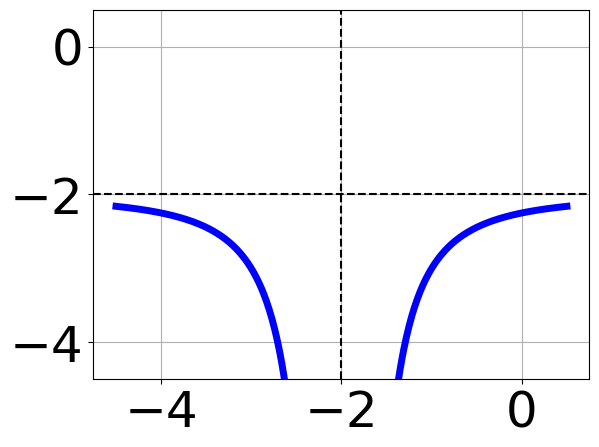
\includegraphics[width = 0.3\textwidth]{../Figures/rationalEquationToGraphAA.png}\item 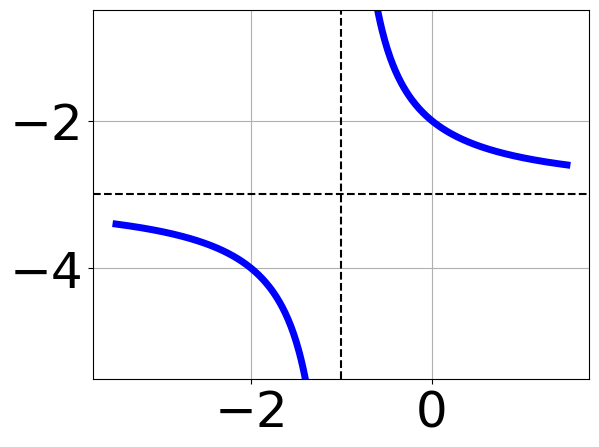
\includegraphics[width = 0.3\textwidth]{../Figures/rationalEquationToGraphBA.png}\item 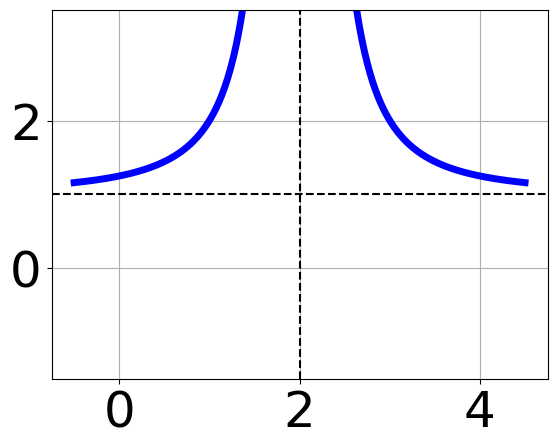
\includegraphics[width = 0.3\textwidth]{../Figures/rationalEquationToGraphCA.png}\item 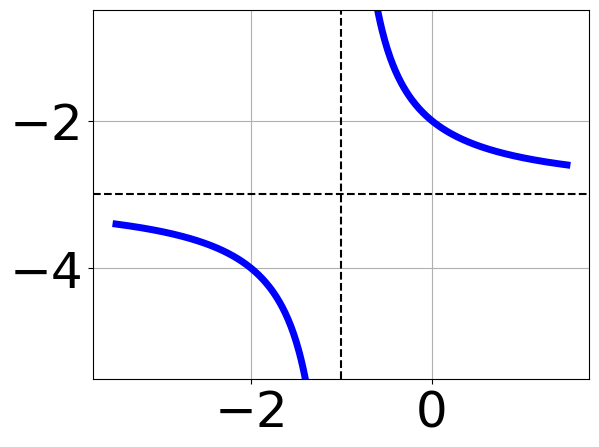
\includegraphics[width = 0.3\textwidth]{../Figures/rationalEquationToGraphDA.png}\end{multicols}\item None of the above.
\end{enumerate} }
\litem{
Solve the rational equation below. Then, choose the interval(s) that the solution(s) belongs to.\[ \frac{-2x}{-2x + 6} + \frac{-3x^{2}}{-12x^{2} +22 x + 42} = \frac{-4}{6x + 7} \]\begin{enumerate}[label=\Alph*.]
\item \( x \in [-2.01,-0.52] \)
\item \( x_1 \in [0.05, 1.45] \text{ and } x_2 \in [-3.2,-0.8] \)
\item \( x \in [-3.39,-1.71] \)
\item \( \text{All solutions lead to invalid or complex values in the equation.} \)
\item \( x_1 \in [0.05, 1.45] \text{ and } x_2 \in [-1.6,4.7] \)

\end{enumerate} }
\end{enumerate}

\end{document}